

\subsection{$\Sigma$-encoding for conformance checking}\label{sec:dadtap}
As per the previous considerations, we want to show that it is sufficient to provide a specific characterization of $\Sigma$, which will be used to generate an automaton accepting symbols in $\Sigma$ and to transform traces as finite sequences in $\Sigma^*$. The proposed approach for obtaining $\Sigma$ from a (data-aware) Declare model $\varphi_{\mathcal{M}}$ is sketched in Figure~\ref{fig:twoexamples}, and described in detail in the following.

\begin{figure}[!t]
	%{\hspace{-1.3cm}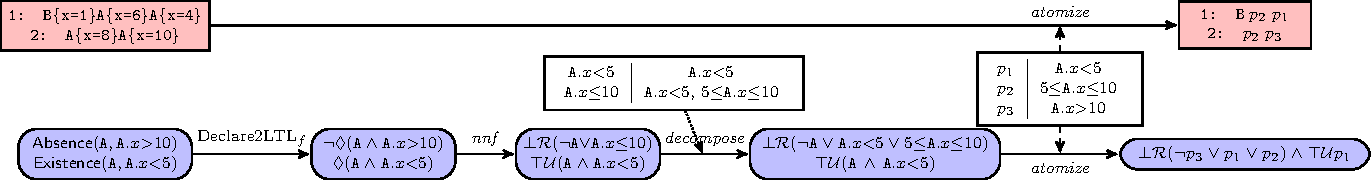
\includegraphics[width=1.3\textwidth]{images/example_1}}
	{\hspace{-1.3cm}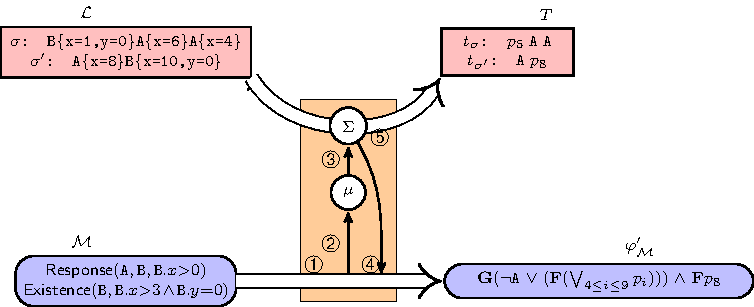
\includegraphics[width=1.3\textwidth]{images/example_3}}
	\caption{Intermediate steps required for obtaining $\Sigma=\Set{p_i|1\leq i\leq 9}\cup\{\texttt{A}\}$ from $\mathcal{M}$ and transforming $\mathcal{L}=\Set{\sigma,\sigma'}$ to a set of finite sequences $T=\Set{t_\sigma,t_{\sigma'}}$, as well as replacing atoms in $\varphi_{\mathcal{M}}$ with equivalent atoms in $\Sigma$ ($\varphi_{\mathcal{M}}'$).}\label{fig:twoexamples}
\end{figure}

In step 1, we exploit the usual conversion of each single Declare clause into an LTL$_f$ formula in the \textit{negated normal form} \cite{LiPZVR20}, where negation is possibly pushed inside atoms ``$\texttt{A}.k\;\Re\; c$'' by replacing $\Re$ with its negation.


In step 2, for each compound condition $\psi=\phi_{\texttt{A}}\wedge \phi^d$ over labels $\texttt{A}\in\textsf{Act}$, we collect all the atoms in $\phi_d$ in the form ``$\texttt{A}.k\;\Re\; c$'' for $k\in K$ in a map $\mu(\texttt{A},k)$. Contextually, we represent each atom as an interval, and we \textit{decompose} them
%
%%We now describe the main contribution of the paper, namely a technique for computing log trace alignments over Declare data-aware models. Our approach takes as input \begin{enumerate*}[label=\emph{\alph*})]
%	\item a Declare data-aware model $\mathcal{M}$ expressed as a set of instantiated templates,
%	\item a log trace $\sigma$,
%\end{enumerate*} and ranks the outcome of a LTL$_f$ conformance checking $\sigma\tilde{\vDash}\varphi$ accordingly to a data distance function $\mathcal{D}$.
%
%%The input transformation for reducing the data-aware alignment problem to the data-agnostic one is presented in Figure~\ref{fig:twoexamples} for two alignment examples. In particular, we first transform the data-aware Declare model, for then collecting the required information for providing the trace transformation.
%
%%\textbf{data-aware Declare Model Processing.}
%
%
%
%
%%In step 3, we collect the data-aware predicates ``$\texttt{A}.\textit{var}\;\Re\;c$'' from all the model's clauses and group them by $\texttt{A}.\textit{var}$; each of these predicates is \textit{decomposed}
into a disjunction of maximal non-overlapping data-aware predicates. This task can be efficiently computed via interval trees \cite{inttree}. E.g., predicates $\texttt{B}.x>3$ and $\texttt{B}.x>0$ are first represented as intervals $\interval({3,+\infty})$ and $\interval({0,+\infty})$, and then decomposed into disjoint sub-invervals $\interval({-\infty,0}]$, $\interval[{0,3}]$, and $\interval({3,+\infty})$. Last, we replace the atoms in each LTL$_f$ formula by its decomposed representation, if any.


In step 3, we put an atom $\texttt{A}\in\textsf{Act}$ in $\Sigma$ if the map $\mu(\texttt{A},k)$ is empty for each key $k\in K$; otherwise, given all the keys $k_{\texttt{A}_1},\dots,k_{\texttt{A}_h}\in K$ for which the map $\mu(\texttt{A},k_{\texttt{A}_i})$ is not empty, we partition the data space by combining the non-overlapping intervals as $\mu(\texttt{A},k_{\texttt{A}_1})\times\cdots\times\mu(\texttt{A},k_{\texttt{A}_h})$ obtained from the previous step. For each of this interval combination, we generate a fresh atom and put it in $\Sigma$. E.g., label \texttt{A} is never associated to a data condition, and therefore it will be associated to one single atom \texttt{A}. Concerning the label \texttt{B}, it is associated to data intervals over keys $x$ and $y$, which induce a space partitioning of 9 intervals, for which we generate distinct atoms $p_1\dots p_9$. As a result, we obtain $\Sigma=\Set{p_i|1\leq i\leq 9}\cup\Set{\texttt{A}}$.


%In step 4, for each event label \texttt{A}, we partition the data space \textit{var}$_1\times\dots\times$\textit{var}$_h$ associated to \texttt{A} by exploiting the disjoint intervals mined in the previous step. Each of such combination will be syntactically represented as a fresh \textit{atom}  proposition $p_i$: this implies that the label \texttt{A} is represented by the disjunction $\bigvee_ip_i$. When the data space associated to the predicates mined for \texttt{A} has only one property,  the atoms corresponds to the ones mined in the previous step. E.g., \texttt{A} in the first example from \ref{fig:twoexamples} is equivalent to $p_1\vee p_2\vee p_3$, and $\texttt{A}.\textit{x}<5$ is rewritten as $p_1$; given that such atoms represent disjoint intervals, then $\texttt{A}\wedge p_1\equiv p_1$. Similarly, $\neg \texttt{A}\vee \texttt{A}.\textit{x}<5\vee 5\leq\texttt{A}.\textit{x}\leq 10$ can be immediately rewritten as $\neg(p_1\vee p_2\vee p_3)\vee p_1\vee p_2$, which is equivalent to $\neg p_3\vee p_1\vee p_2$. Last, each LTL$_f$ representation of a data-aware Declare clause is represented into one single LTL$_f$ formula by conjunction and simplification.

Given the previously generated atoms, we can now generate a finite sequence $t_\sigma\in T$ for each log trace $\sigma\in\mathcal{L}$, and replace the compound conditions in the LTL$_f$ interpretation $\varphi_{\mathcal{M}}$ of model $\mathcal{M}$ with a disjunction of atoms from $\Sigma$ as described in \S\ref{sec:wa}, thus obtaining an equivalent LTL$_f$ formula $\varphi_{\mathcal{M}}'$.
%
%\textbf{data-aware Log Trace Processing.} Given the atomization in Step 4, we process each data-enriched event within the trace as follows: if the event label is never associated with a data predicate, then we just discard the data information; otherwise, we replace each event with the single corresponding atom satisfying the associated semantics. Please observe that, by previous construction, each event can be represented by just one possible propositional atom, as the previous construction guarantees a partitioning (thus non-overlapping) representation of the data space.
E.g., all the trace events from Figure~\ref{fig:twoexamples} labelled as \texttt{A} are replaced with the atom \texttt{A}, as there are no (data) conditions in the model $\mathcal{M}$ that we can exploit to partition the data space. On the other hand, each data condition \texttt{B} is replaced by an equivalent atom in $\Sigma$: event \texttt{B\{x=1,y=0\}} is uniquely represented by $p_5$, while event \texttt{B\{x=10,y=0\}} is uniquely represented by atom $p_8$. Similar considerations can be drawed for the $\psi$ compound atoms in $\varphi_{\mathcal{M}}$ where compound conditions are replaced into an equivalent disjunction of atoms in $\Sigma$: $\texttt{B}.x>0$ will be described by all the possible configurations of $y$ and data intervals $0<\texttt{B}.x\leq 3$ and $\texttt{B}.x>3$, which are identified by the disjunction $p_4\vee p_5\vee p_6\vee p_7\vee p_8\vee p_9$. On the other hand, $\texttt{B}.x>3\wedge \texttt{B}.y=0$ can be directly mapped to atom $p_8$: this results into generating an equivalent formula $\varphi_{\mathcal{M}}'$ out of $\varphi_{\mathcal{M}}$.

After generating $\varphi_{\mathcal{M}}'$, we can exploit directly existing approaches \cite{LeoniMA12,Westergaard11,Lydia} to generate DFAs, thus obtaining Figure \ref{fig:g1g2}: the first trace will be never accepted by the model, as well as the first sequence is never accepted by the associated automaton. Similarly, the second trace is accepted by the model, as well as the second sequence is accepted by the DFA. In the forthcoming subsection, we will discuss how to generate repaired sequences that are accepted by the model.

\subsection{Automaton Manipulation for Trace Alignment}\label{ssec:amfta}
Let us now consider a string sequence $t_\sigma=t_1\cdots t_n$ generated from a log trace $\sigma$ in the previous section, and the constraint automaton $\mathcal{A}_{\varphi_{\mathcal{M}}}$ generated from the Declare model $\mathcal{M}$, both generated via a set of atoms $\Sigma$. If the trace was deviant with respect to the model, we are interested in generating a repair sequence $\varrho=\varrho_1\cdots \varrho_m$ from $t_\sigma$ describing the operations to perform over $\sigma$ to make it conformant to the model $\mathcal{M}$.

To realize this transformation, we consider two kinds of atomic violations, which can be caused by wrong (\textit{deletion}) or missing (\textit{insertion}) activities with data conditions in $\Sigma$. Differently from the non-data aware contexts such as \cite{XuLZ17a,MaggiMCA18}, we also need to model \textit{replacement} operations, defined as data updates within one single trace event: these can be mimicked by delete operations followed by insertion ones, as they substitute an event within a trace violating the model  with a conforming one. Such operations can be defined as follows:
\begin{itemize}
	%\item synchronization $[\sigma_k\leftrightarrow \phi]$ aborts if $\sigma_k\neq\phi$, for  $1\leq k\leq |\sigma|$
	\item \textit{deletion}\,\, $[\#\sigma_k\leftarrow \phi]::= \sigma_1\cdots\sigma_{k-1}\sigma_{k+1}\cdots \sigma_n$,\,\,\, for $n=|\sigma|$, $1\leq k\leq n$, and $\phi=\sigma_k$
	\item \textit{insertion} $[@\sigma_k\leftarrow \phi]::= \sigma_1\cdots\sigma_{k-1}\phi\sigma_{k}\cdots \sigma_n$,\,\,\,\,\,\,\,\,\,\,\,\,\, for $n=|\sigma|$ and $1\leq k\leq n$
	\item \textit{replacement} $[\sigma_k[\phi\mapsto\phi']]::=\sigma_1\cdots \sigma_{k-1}\phi'\sigma_{k+1}\cdots\sigma_n$ for $n=|\sigma|$, $1\leq k\leq n$, and $\phi=\sigma_k$
\end{itemize}
Each of these operations has an associated cost, either quantifying the severity of the found violation or determining which operations shall be preferred. E.g., by assigning a higher cost to insertions and deletions and a lower one to replacements, we will favor replacements when possible. The \textit{transformation cost} is defined as the number of deletions multiplied by their cost, plus the number of insertions multiplied by their cost, plus the number of replacements multiplied by their cost.

We can now define the conformance checking problem as follows:
\begin{definition}[Log/Declare Conformance Checking]
Given a trace $\sigma$ and a Declare model $\mathcal{M}$, either $\sigma$ conforms to $\mathcal{M}$, or $\sigma$ is deviant and it exists a repair sequence $\varrho$ both making $\sigma$ non-deviant for $\mathcal{M}$ and guaranteeing a minimal transformation cost.
\end{definition}

%\texttt{\color{red}[TODO]} we consider insertions and deletions as possible repairs, while substitutions can be modeled by deletions followed by insertions. Synchronizations are \texttt{noops} requiring that a trace $\sigma$ at step $k$ contains a predicate $\phi$.
%%
%Therefore, any repair  of a trace $\sigma$ can be expressed in terms of a sequence of operations $\texttt{op}_1\cdots \texttt{op}_m$ which, when executed in appearance order, generate a novel trace $\tilde{\sigma}$ from $\sigma$.  \texttt{\color{red}[TODO]}
%%
%
%Last, the amount of repairs can be numerically quantified using a cost function $\mathcal{C}$ returning zero for any synchronization and $1$ otherwise; therefore $cost(\sigma, \tilde{\sigma})$ returns the minimal number of non-synchronization operations\footnote{Formally, $cost(\sigma,\tilde{\sigma})=\min_{\substack{\texttt{op}_1\cdots \texttt{op}_m,\\(\texttt{op}_m\,\circ \cdots\circ\, \texttt{op}_1)(\sigma)=\tilde{\sigma}}}\sum_{1\leq i\leq m}\mathcal{C}(\texttt{op}_m)$} required to obtain $\tilde{\sigma}$ from $\sigma$. Therefore, the conformance checking of a log trace $\sigma$ against a  Declare model represented as an LTL$_f$ formula $\varphi$ as in \cite{XuLZ17a} either returns $\sigma$ with cost zero if $\varphi\vDash\varsigma$ or, otherwise, returns a set of pairs $\Set{\braket{\tilde{\sigma},\texttt{op}_1\cdots\texttt{op}_m}_i}_{1\leq i\leq k, k\in\mathbb{N}}$, where\footnote{Formally, $\sigma\tilde{\vDash}\varphi = \Set{\braket{\tilde{\sigma},\texttt{op}_1\cdots\texttt{op}_m} | cost(\sigma,\tilde{\sigma}) = \min_\mu cost(\sigma,\mu),\;\tilde{\sigma}\vDash\varphi,\; (\texttt{op}_m\,\circ \cdots\circ\, \texttt{op}_1)(\sigma)=\tilde{\sigma}}$.} each trace $\tilde{\sigma}\in S$ is conformant to $\varphi$ and minimizes the alignment cost $cost(\sigma,\tilde{\sigma})$ via a repair sequence $\texttt{op}_1\cdots\texttt{op}_m$. We denote the output of such conformance checking as $\sigma\tilde{\vDash}\varphi$.

The process of generating a repair sequence can be addressed by resorting to DFAs (\S\ref{sec:wa}). Let $t_\sigma=t_1\cdots t_n$ be a string sequence generated from a log trace $\sigma$ via $\Sigma$, $\mathcal{A}_{\varphi_{\mathcal{M}}}=(\Sigma,Q,q_0,\rho,F)$ the constraint automaton to check $t_\sigma$ against. From $t_\sigma$, we define a further automaton, called the \textit{path automaton} $\mathcal{T}=(\Sigma_t,Q_t,q_0^t,\rho_t,F_t)$ having \begin{enumerate*}[label=\emph{\alph*})]
	\item $\Sigma_t=\Set{t_i|t_i\in t_\sigma}$,
	\item $Q_t=\Set{q_0^t,\cdots,q_n^t}$ as a set of $|t_\sigma|+1$ states,
	\item $\rho(q_i^t,e_{i+1})=q_{i+1}^t$ for $0\leq i\leq n-1$,
	and
	\item $F_t={q_n^t}$.
\end{enumerate*} By definition, such graph accepts only $t_\sigma$.

\begin{figure}[!t]
	\centering
	{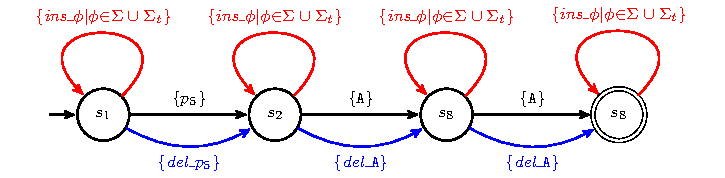
\includegraphics[width=.7\textwidth]{images/Tplus}}
	\caption{Augmented path automaton $\mathcal{T}^+$ for $t_{\sigma'}=p_5\;\texttt{A}\;\texttt{A}$.}\label{fig:tplus}
\end{figure} \begin{figure}[!t]
\centering
{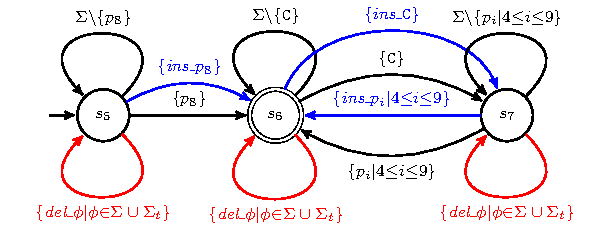
\includegraphics[width=.7\textwidth]{images/Aplus}}
\caption{Augmented path automaton $\mathcal{A}_{\varphi_{\tiny\mathcal{M}}}^+$ for $\mathcal{A}_{\varphi_{\tiny\mathcal{M}}}$.}\label{fig:aplus}
\end{figure}
Next, we augment $\mathcal{T}$ and $\mathcal{A}_{\varphi_{\mathcal{M}}}$ by adding transitions related to just the atomic operations of insertions and deletions: Thus, from $\mathcal{T}$ we generate the automaton $\mathcal{T}^+=(\Sigma_t^+,Q_t,q_0^t,\rho_t^+,F_t)$ having:
\begin{itemize}
	\item $\Sigma_t^+$ extending $\Sigma_t\subseteq \Sigma$ by adding an insertion $\textit{ins\_}\phi$ for each atom $\phi\in\Sigma_t\cup\Sigma$ and a deletion $\textit{del\_}\phi$ for each atom  $\phi\in\Sigma_t$.
	\item $\rho_t^+$ extending $\rho_t$ by adding deletions $\rho_t^+(p,\textit{del\_}\phi)=q$ for each transition $\rho_t(p,\phi)=q$; and, for all atoms $\phi\in\Sigma\cup\Sigma_t$ and states $q\in Q_t$, we add insertions $\rho_t^+(q,\textit{ins\_}\phi)=q$.
\end{itemize}
Figure~\ref{fig:tplus} shows the path automaton generated from the deviant trace $\sigma_1$ from Figure~\ref{fig:twoexamples}. Similarly, from $\mathcal{A}_{\varphi_{\mathcal{M}}}$ we obtain $\mathcal{A}_{\varphi_{\tiny\mathcal{M}}}^+=(\Sigma^+,Q,q_0,\rho^+,F)$ having:
\begin{itemize}
	\item $\Sigma^+$ extending $\Sigma$ by adding an insertion $\textit{ins\_}\phi$ for each atom $\phi\in\Sigma$ and a deletion $\textit{del\_}\phi$ for each atom  $\phi\in\Sigma\cup\Sigma_t$.
\item $\rho^+$ extending $\rho_t$ by adding insertions $\rho^+(p,\textit{ins\_}\phi)=q$ for each transition $\rho(p,\phi)=q$; and, for all atoms $\phi\in\Sigma\cup\Sigma_t$ and states $q\in Q$, we add deletions $\rho_t^+(q,\textit{del\_}\phi)=q$.
\end{itemize}
Figure~\ref{fig:aplus} shows the automaton augmented with the repair operations $\mathcal{A}_{\varphi_{\tiny\mathcal{M}}}^+$ obtained for the Declare model $\mathcal{M}$ in Figure~\ref{fig:twoexamples} via $\Sigma$. Intuitively, $\mathcal{A}_{\varphi_{\tiny\mathcal{M}}}^+$ accepts all the string sequences conformant to the model and have been obtained by adding/removing the missing/wrong atoms to/from $t_\sigma$, where atomic operations are explicitly marked. As required, both augmented automatons will never accept $t_{\sigma'}=p_5\;\texttt{A}\;\texttt{A}$. However, if we repair the sequence by adding $p_8$ at the end and explicitly remarking such repair with $\textit{ins\_}p_8$, then all the augmented automata will accept $\hat{t_{\sigma'}}=p_5\;\texttt{A}\;\texttt{A}\;\textit{ins\_}p_8$.

Next, we show how automated planners searching for the repair operations $\varrho$ that are going to be exploited to repair the trace $\sigma$ via the previously designed automata.

\subsection{Encoding in PDDL}\label{ssec:eip}
\texttt{\color{red}[TODO]}
\\

E.g., the alignment result $\hat{t_\sigma}=p_5\;\texttt{A}\;\texttt{A}\;\textit{ins\_}p_8$ of trace $\sigma=$\texttt{B\{x=1,y=0\}A\{x=6\}\\A\{x=4\}} generates the repair $\varrho=[@\sigma_4\leftarrow p_8]$ after removing the \texttt{sync} operations.

\subsection{Trace repair}\label{ssec:trerepair}
Last, we need to leverage the repair actions generated by the planner to repair the data trace. In particular, the generated repair actions are always ordered and incrementally change different positions within the trace. By removing all the \texttt{sync}s from the planner, we will obtain a sequence of insertion $[@\sigma_k\leftarrow \phi]$, deletion $[\#\sigma_k\leftarrow \phi]$, and replacement $[\sigma_k[\phi\mapsto \phi']]$ operations for a trace $\sigma$ via is associated $t_\sigma$. While deletions $[\#\sigma_k\leftarrow \phi]$ can be trivially implemented in the data-aware scenario by simply removing the problematical event at position $k$ from $\sigma$, for insertions and replacements we need to add events with their associated payloads or adapt such values. Replacements $[\sigma_k[\phi\mapsto \phi']]$ can be easily be implemented by replacing the values in $\sigma_k$ violating data conditions $\phi'$ expressed with a conjunction of data intervals over different keys with the nearest values in $\phi'$ to the values in $\sigma_k$. On the other hand, insertions require to generate totally new values: given that traces $\sigma=\sigma_1\dots \sigma_n$ model temporal activities starting at $\sigma_1$ and ending at $\sigma_n$,  the insertion $[@\sigma_k\leftarrow \phi]$ of a new event compliant with $\phi$ at position $k$ can be modeled by generating a new event having the trace label \texttt{A} induced by $\phi$, which is then instantiated with the same data values present in the last occurrence of an event similarly labeled (i.e., \texttt{A}) if any, and instantiated with default values otherwise; next, such values are repaired by choosing the values in $\phi$ nearer to the one in the newly added event.

E.g., given the repair $\varrho=[@\sigma_4\leftarrow p_8]$ generated for a trace $\sigma=$\texttt{B\{x=1,y=0\}\\A\{x=6\}A\{x=4\}}, we obtain a new trace $\sigma=$\texttt{B\{x=1,y=0\}$  $A\{x=6\}A\{x=4\}B\{x=4,y=0\}}, where \texttt{4} is the nearest integer to \texttt{B.x=1} from the first event which is compliant to $p_8\equiv\texttt{B}.x>3\wedge \texttt{B}.y=0$. 